\documentclass[12pt]{article}

\usepackage{answers}
\usepackage{setspace}
\usepackage{graphicx}
\usepackage{enumitem}
\usepackage{multicol}
\usepackage{mathrsfs}
\usepackage[margin=1in]{geometry} 
\usepackage{amsmath,amsthm,amssymb}
\usepackage{pgfplots}
\pgfplotsset{compat=1.15}
 
\newcommand{\N}{\mathbb{N}}
\newcommand{\Z}{\mathbb{Z}}
\newcommand{\C}{\mathbb{C}}
\newcommand{\R}{\mathbb{R}}

\DeclareMathOperator{\sech}{sech}
\DeclareMathOperator{\csch}{csch}
 
\newenvironment{theorem}[2][Theorem]{\begin{trivlist}
\item[\hskip \labelsep {\bfseries #1}\hskip \labelsep {\bfseries #2.}]}{\end{trivlist}}
\newenvironment{definition}[2][Definition]{\begin{trivlist}
\item[\hskip \labelsep {\bfseries #1}\hskip \labelsep {\bfseries #2.}]}{\end{trivlist}}
\newenvironment{proposition}[2][Proposition]{\begin{trivlist}
\item[\hskip \labelsep {\bfseries #1}\hskip \labelsep {\bfseries #2.}]}{\end{trivlist}}
\newenvironment{lemma}[2][Lemma]{\begin{trivlist}
\item[\hskip \labelsep {\bfseries #1}\hskip \labelsep {\bfseries #2.}]}{\end{trivlist}}
\newenvironment{exercise}[2][Exercise]{\begin{trivlist}
\item[\hskip \labelsep {\bfseries #1}\hskip \labelsep {\bfseries #2.}]}{\end{trivlist}}
\newenvironment{solution}[2][Solution]{\begin{trivlist}
\item[\hskip \labelsep {\bfseries #1}]}{\end{trivlist}}
\newenvironment{problem}[2][Problem]{\begin{trivlist}
\item[\hskip \labelsep {\bfseries #1}\hskip \labelsep {\bfseries #2.}]}{\end{trivlist}}
\newenvironment{question}[2][Question]{\begin{trivlist}
\item[\hskip \labelsep {\bfseries #1}\hskip \labelsep {\bfseries #2.}]}{\end{trivlist}}
\newenvironment{corollary}[2][Corollary]{\begin{trivlist}
\item[\hskip \labelsep {\bfseries #1}\hskip \labelsep {\bfseries #2.}]}{\end{trivlist}}
 
\begin{document}
 
% --------------------------------------------------------------
%                         Start here
% --------------------------------------------------------------
 
\title{Problem Set 2}%replace with the appropriate homework number
\author{Basil R. Yap\\ %replace with your name
40.316 Game Theory - Term 8} %if necessary, replace with your course title
 
\maketitle
%Below is an example of the problem environment

% Question 1
\begin{figure}[h!]
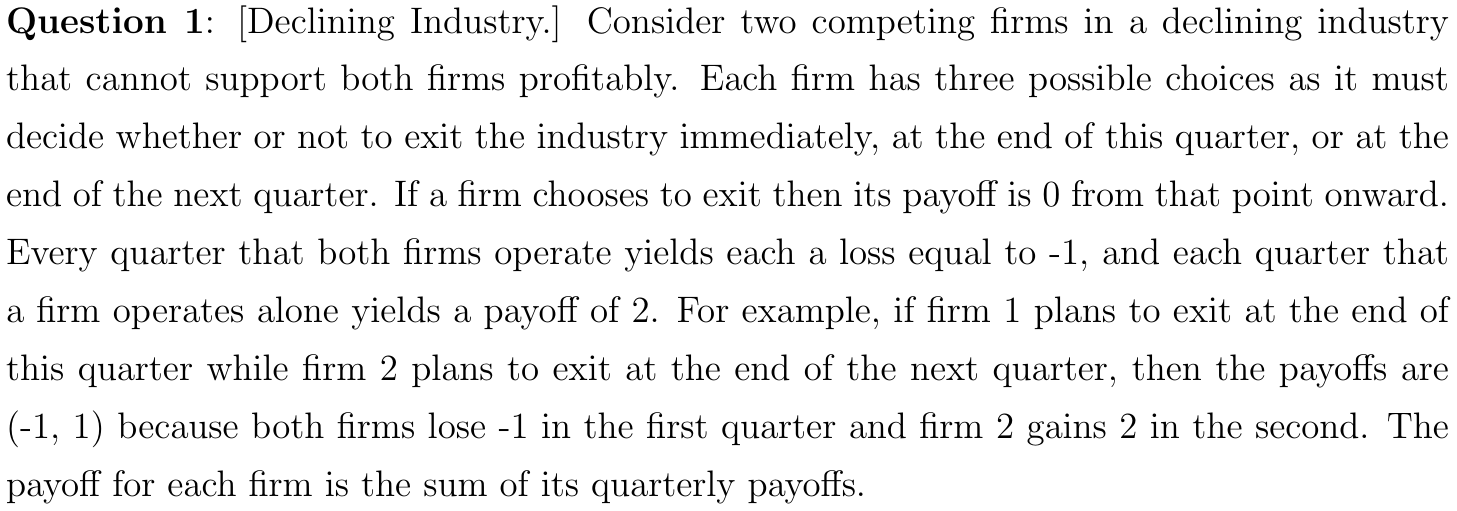
\includegraphics[width=\linewidth]{./assets/201806021724.png}
\end{figure}
\begin{enumerate}[label=(\alph*)]
\item Write down this game in matrix form
\item Is there any pure strategy that is dominated by some mixed strategy? Why?
\item Find the pure strategy Nash equilibria.
\item Find the unique mixed strategy Nash equilibrium (hint: you can use your answer to (b) to make things easier).
\end{enumerate}

\begin{solution}{}~\\
\begin{enumerate}[label=(\alph*)]
\item
\item 
\item 
\item 
\end{enumerate}
\end{solution}

% Question 2
\begin{figure}[h!]
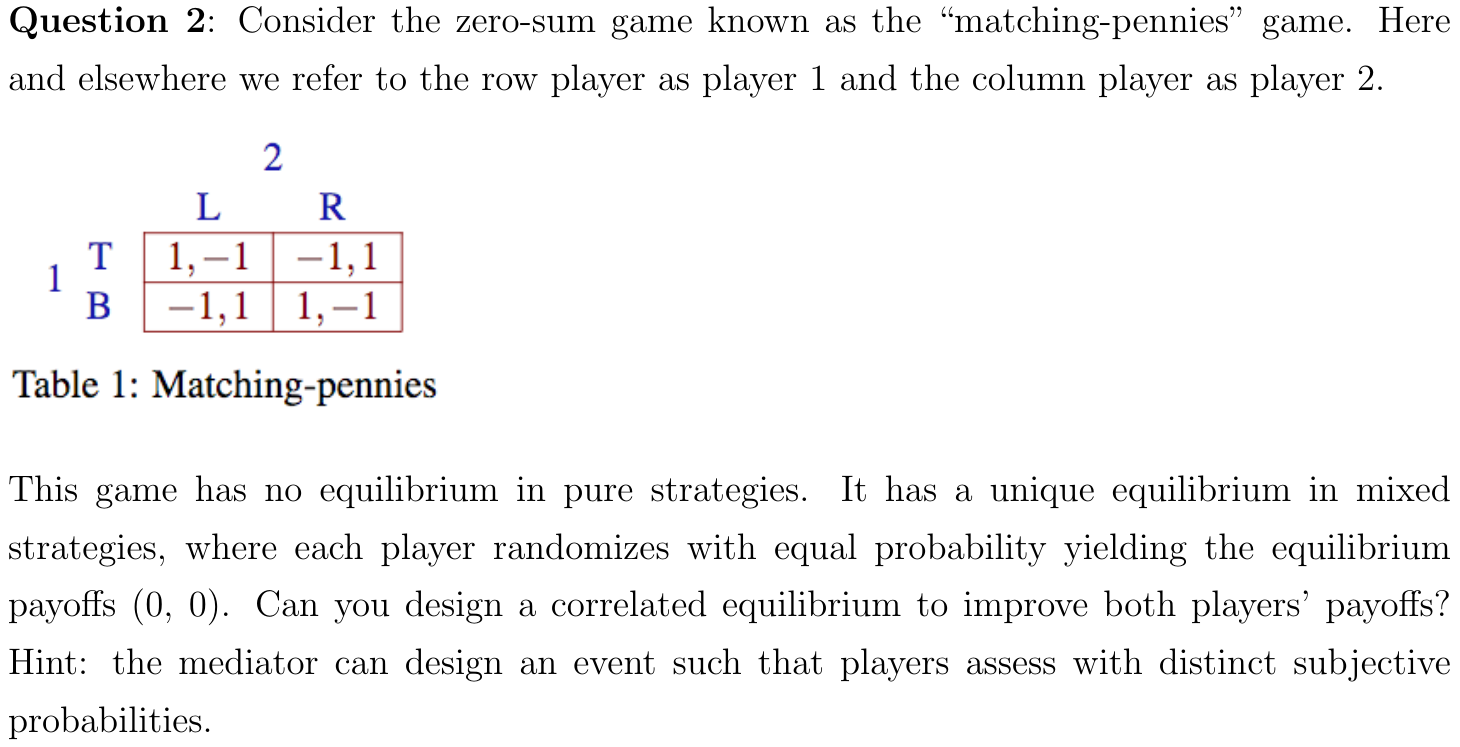
\includegraphics[width=\linewidth]{./assets/201806021725.png}
\end{figure}

\begin{solution}{}~\\

\end{solution}

% Question 3
\begin{figure}[h!]
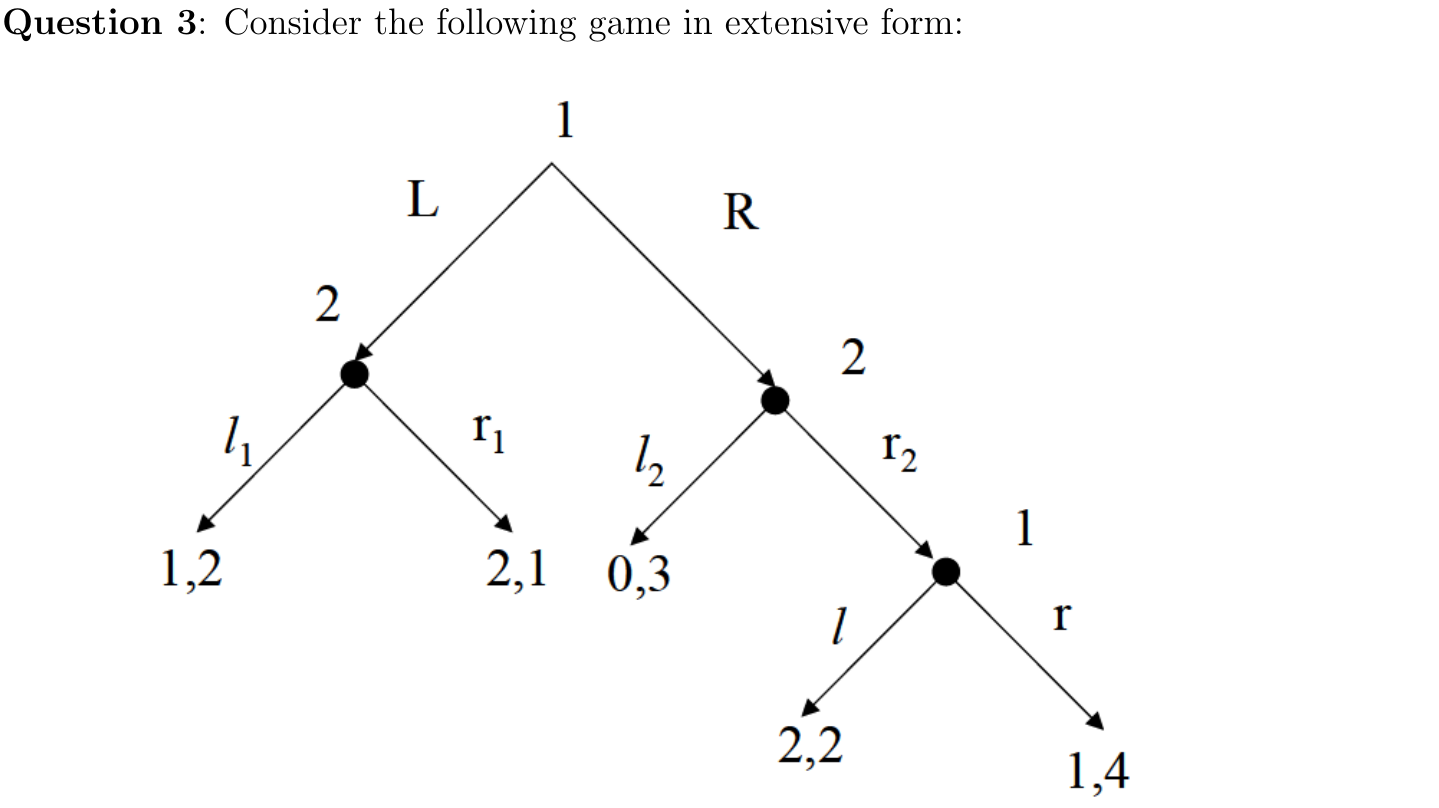
\includegraphics[width=\linewidth]{./assets/201806021726.png}
\end{figure}
\begin{enumerate}[label=(\alph*)]
\item Apply backwards induction in this game and find the subgame perfect equilibrium of the game
\item Write the game in normal-form and find the set of pure strategy Nash equilibria.
\end{enumerate}

\begin{solution}{}~\\
\begin{enumerate}[label=(\alph*)]
\item 
\item
\end{enumerate}
\end{solution}

% Question 4
\begin{figure}[h!]
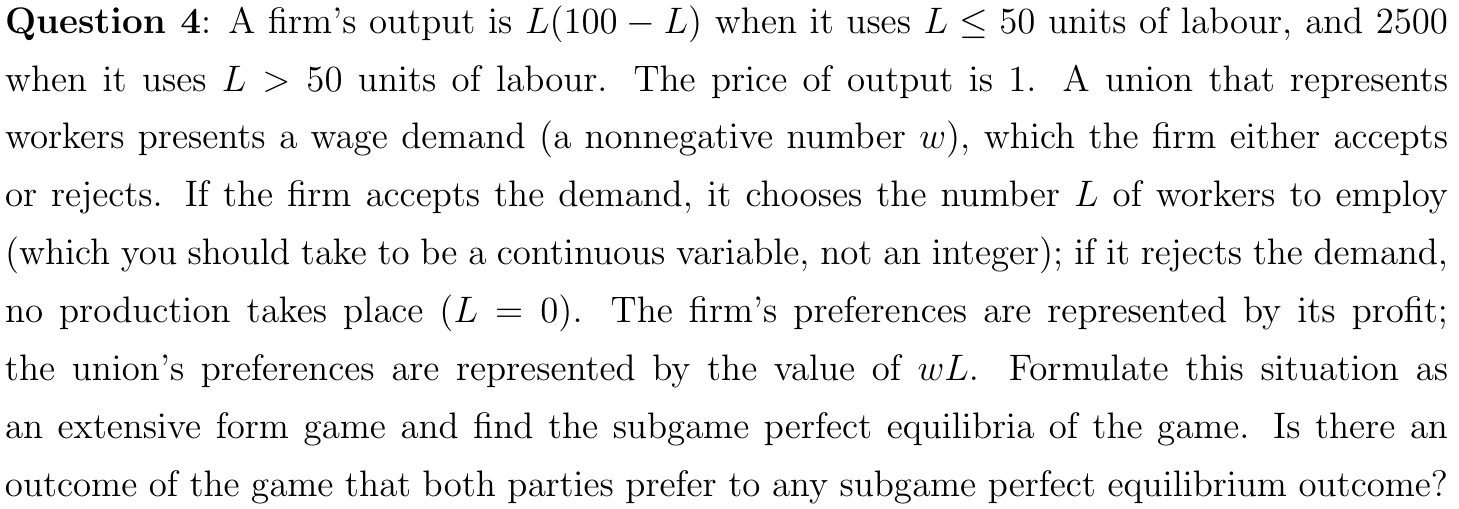
\includegraphics[width=\linewidth]{./assets/201806021727.png}
\end{figure}

\begin{solution}{}~\\

\end{solution}

% Question 5
\begin{figure}[h!]

\includegraphics[width=\linewidth]{./assets/201806021728.png}
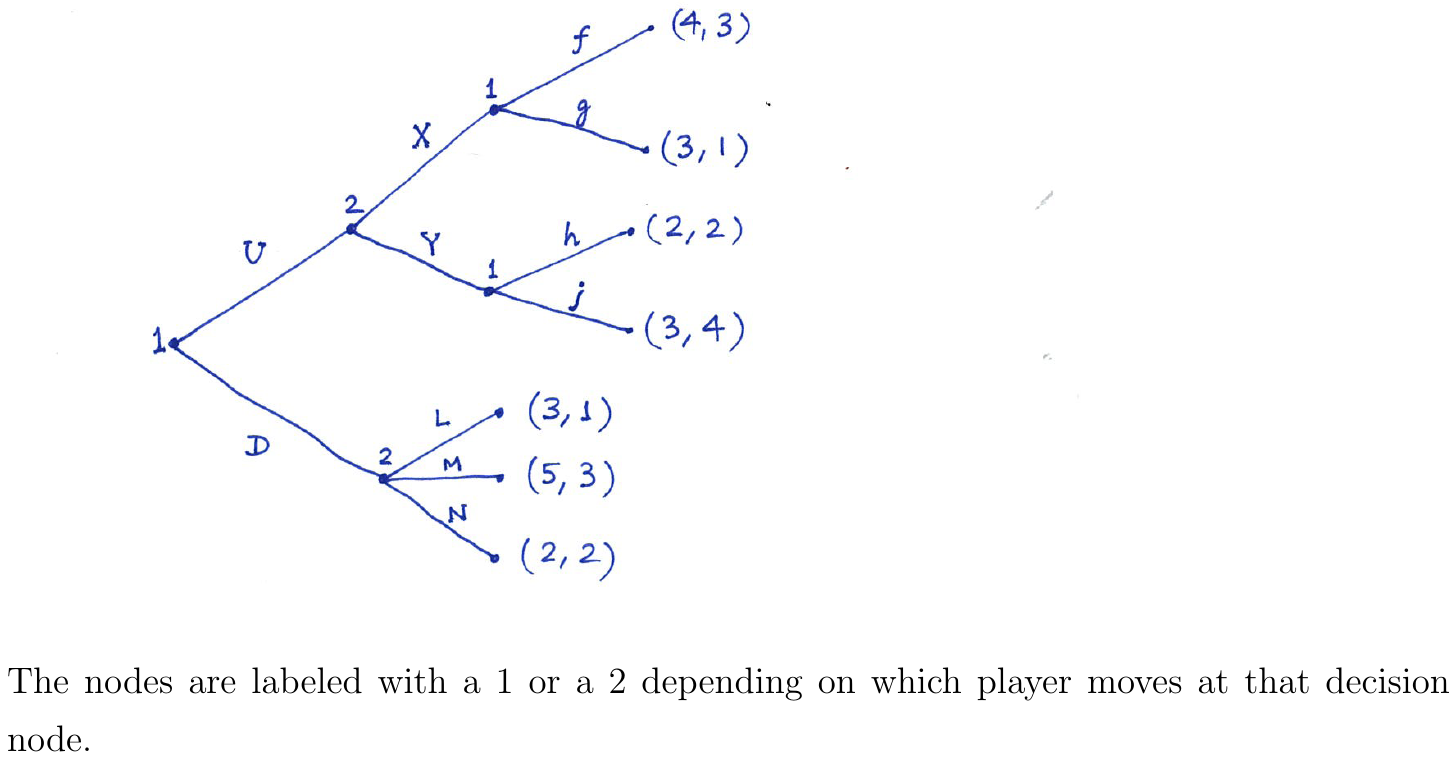
\includegraphics[width=\linewidth]{./assets/201806021729.png}
\end{figure}
\begin{enumerate}[label=(\alph*)]
\item Find a subgame perfect equilibrium (in pure strategies).
\item Is there a Nash equilibrium for the game that is not SPE? If yes, write down one such equilibrium.
\end{enumerate}

\begin{solution}{}~\\
\begin{enumerate}[label=(\alph*)]
\item 
\item 
\end{enumerate}
\end{solution}

% Question 5
\begin{figure}[h!]
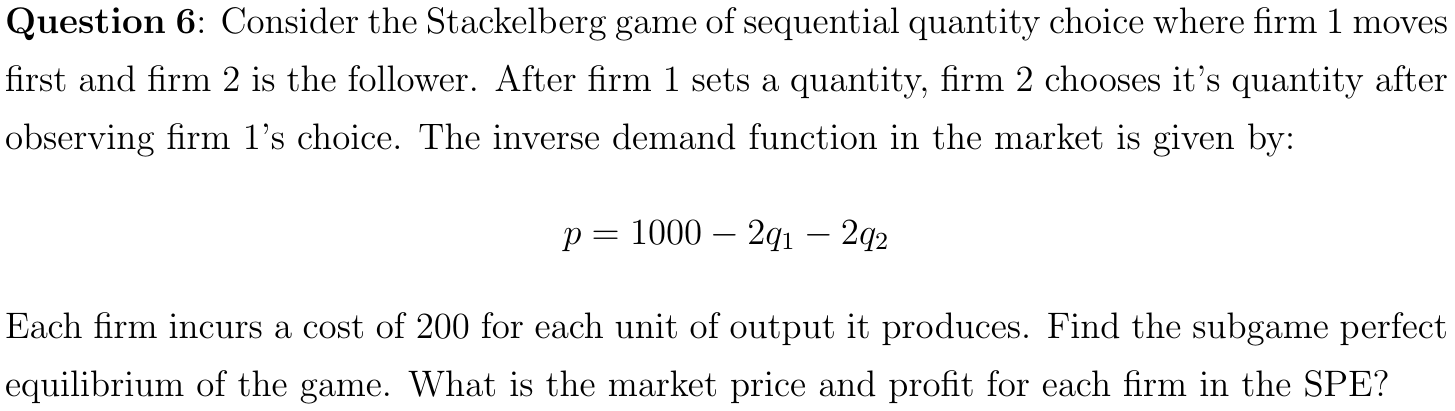
\includegraphics[width=\linewidth]{./assets/201806021730.png}
\end{figure}

\begin{solution}{}~\\

\end{solution}

\end{document}
